\documentclass{article}
\usepackage{amsmath,amssymb}
\usepackage{tikz}
\usetikzlibrary{arrows.meta,positioning,calc,shapes.geometric}
\pagestyle{empty}
\begin{document}
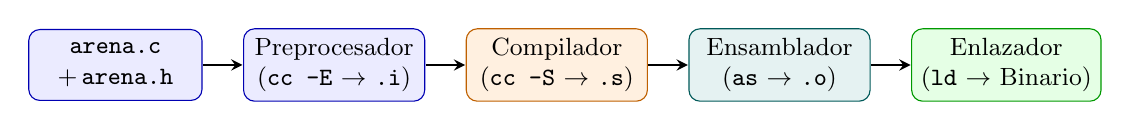
\begin{tikzpicture}
\tikzset{node distance=1.6cm, >=stealth, thick, font=\small}
\node[draw=blue!70!black, fill=blue!8, rounded corners, minimum width=2.2cm, minimum height=0.9cm, align=center] (src) {\texttt{arena.c}\\+\,\texttt{arena.h}};
\node[draw=blue!70!black, fill=blue!8, rounded corners, minimum width=2.3cm, minimum height=0.9cm, align=center, right=0.5cm of src] (cpp) {Preprocesador\\(\texttt{cc -E} $\to$ \texttt{.i})};
\node[draw=orange!75!black, fill=orange!12, rounded corners, minimum width=2.3cm, minimum height=0.9cm, align=center, right=0.5cm of cpp] (cc1) {Compilador\\(\texttt{cc -S} $\to$ \texttt{.s})};
\node[draw=teal!70!black, fill=teal!10, rounded corners, minimum width=2.3cm, minimum height=0.9cm, align=center, right=0.5cm of cc1] (as) {Ensamblador\\(\texttt{as} $\to$ \texttt{.o})};
\node[draw=green!60!black, fill=green!10, rounded corners, minimum width=2.2cm, minimum height=0.9cm, align=center, right=0.5cm of as] (ld) {Enlazador\\(\texttt{ld} $\to$ Binario)};
\draw[->] (src) -- (cpp);
\draw[->] (cpp) -- (cc1);
\draw[->] (cc1) -- (as);
\draw[->] (as) -- (ld);
\end{tikzpicture}
\end{document}
